In diesem Abschnitt werden Regressionsnetzwerke unter Einsatz von Early Stopping evaluiert, wobei erläutert wird, warum diese Methode für 
Klassifikations-netzwerke nicht zielführend ist. Der Fokus liegt hierbei ausschließlich auf Direct Cascade Netzarchitekturen. 
Early Stopping stellt eine Methode dar, die eingesetzt wird, um Overfitting des Modells auf die Trainingsdaten entgegenzuwirken.

Für sowohl die Regressions- als auch die Klassifikationsmodelle wurde LM als Stoppkriterium verwendet. Zusätzlich kamen bei der 
Regression die MAEM und bei der Klassifikation die ACCM als Metriken zum Einsatz.

\begin{figure}[htpb]
    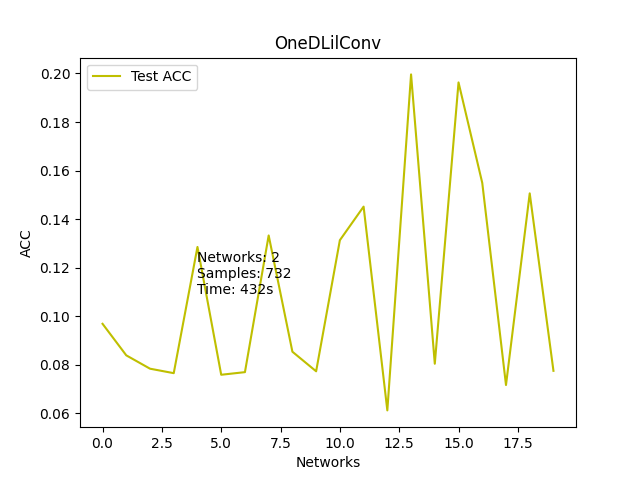
\includegraphics[height=4.5cm]{../../Plots/ba_plots/earlystopping/lossmetric/1dconv_ts.png}
    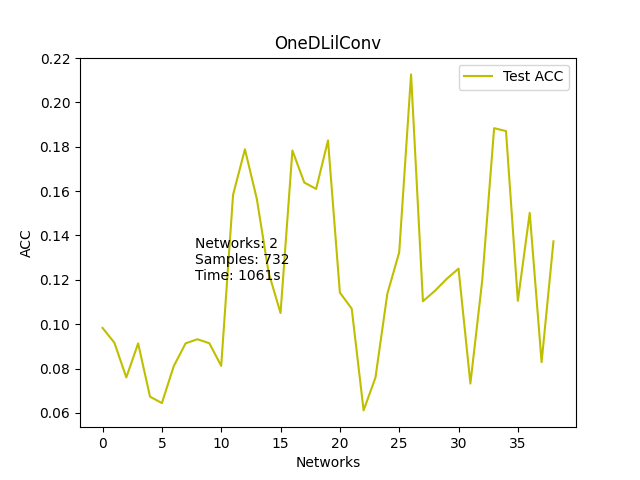
\includegraphics[height=4.5cm]{../../Plots/ba_plots/earlystopping/intermetric/1dconv_ts.png}
    \caption{\label{fig:1dconvmetrics} 
    \small{Hier werden die Testergebnisse für das 1DC-Netzwerk unter Verwendung von Early Stopping dargestellt. Deutlich erkennbar ist, dass sich 
    die Modellleistung durch Early Stopping nicht verbessert. Die exakten Testbezeichnungen lauten: links 1DC:LM/732/10 und rechts 1DC:ACCM/732/10}}
\end{figure}

Bei den Klassifikationsnetzen führt das Early Stopping auf Basis von ACCM nur gelegentlich zu einem vorzeitigen Abbruch des Trainings, ohne 
jedoch eine Verbesserung der Modellleistung zu bewirken. Unter Verwendung von LM tritt dieser Abbruch häufiger auf, was zu einer schnelleren 
Trainingskonvergenz führt. Dennoch bleibt die Leistung der kaskadierten Klassifikationsnetzwerke derart unzureichend, dass ein praktischer 
Einsatz ausgeschlossen ist. Die Ineffektivität von sowohl LM als auch ACCM in diesem Kontext wird anschaulich in 
Abbildung \ref{fig:1dconvmetrics} dargestellt. Hervorzuheben ist, dass ACCM die einzige der betrach-teten Metriken ist, bei der ein Maximum 
angestrebt wird.

Daher erfolgt im Folgenden eine vertiefte Analyse des Regressionsnetzwerks 1Lay. Dabei zielen die verwendeten Metriken, LM und MAEM, auf eine 
Mini-mierung des Fehlermaßes ab.

\begin{figure}[htpb]
    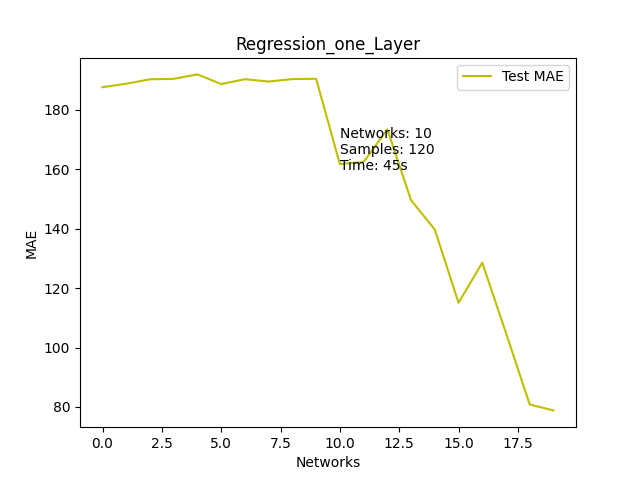
\includegraphics[height=4.5cm]{../../Plots/ba_plots/earlystopping/lossmetric/onelayer_ts.png}
    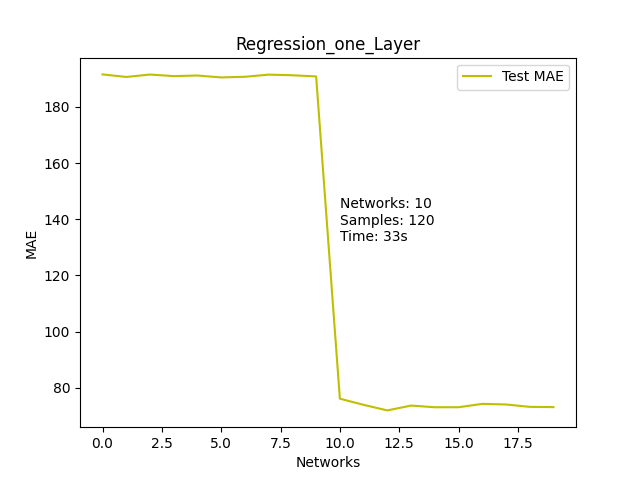
\includegraphics[height=4.5cm]{../../Plots/ba_plots/earlystopping/intermetric/onelayer_ts.png}
    \caption{\label{fig:onelayermetrics} 
    \small{Hier sind die Testergebnisse des 1Lay-Netzwerks unter Verwendung von Early Stopping veranschaulicht. Es zeigt sich, 
    dass die Modellperformanz mit Early Stopping schlechter ausfällt als ohne. 
    Obwohl es in einigen Fällen zu vorzeitigen Trai-ningsabbrüchen kam, wurde dadurch Overfitting nicht entscheidend verhindert. 
    Die eingesetzten Metriken erweisen sich somit als ineffektiv. 
    Die genauen Bezeichnungen der Testläufe lauten: links 1Lay:LM/120/10 und rechts 1Lay:MAEM/120/10.}}
\end{figure}

Die Anwendung der Early-Stopping-Metriken LM und MAEM liefert zwar teilweise akzeptable Ergebnisse, jedoch sind diese deutlich schlechter als die 
Resultate eines Trainings ohne Early Stopping, wie aus den Werten in Abbildung \ref{fig:onelayermetrics} ersichtlich ist.

Die Qualität der erzielten Ergebnisse entspricht in etwa der, als hätte das 1Lay-Netzwerk in der Kaskadenversion mit einer geringen Anzahl an 
Target-Daten direkt auf diese trainiert. Die unzureichende Leistung der Early-Stopping-Metriken ist darauf zurückzuführen, dass sie keine temporären 
Verschlechterungen im Validierungsdatensatz tolerieren und das Training bei der ersten beobach-teten Verschlechterung abbrechen. Dadurch wird 
häufig nicht das tatsächliche Minimum des Fehlermaßes über den augmentierten Vektor weitergegeben, sondern lediglich ein leicht abweichender 
Wert.

Zudem sind diese Metriken nicht in der Lage, ein globales Minimum zu identifizieren, wenn das Trainingsverfahren in einem lokalen Minimum 
verharrt. In einem solchen Fall führt das Early Stopping dazu, dass das Modell im lokalen Minimum verbleibt, anstatt weiter zu 
optimieren.
